%! TEX program = xelatex
\documentclass{beamer}

\usepackage{xeCJK}
\usepackage[utf8]{inputenc}
\usepackage{utopia}
\usepackage{amsmath}
\usepackage{latexsym}
\usepackage{calc}
\usepackage{xcolor}
\usepackage{arydshln}
\usepackage{amssymb}
\usepackage{booktabs}
\usepackage{graphicx}
\usepackage{subcaption}
\usepackage{bookmark}
\usepackage{float}
\usepackage{bm}
\usepackage{bbold}
\usepackage{extarrows}
\usepackage{multirow}

% Color Support
\usepackage{xcolor}
\definecolor{commcolor}{rgb}{0,0.6,0}
\definecolor{rulesepcolor}{rgb}{0.2,0.2,0.2}
\definecolor{stringcolor}{rgb}{0.58,0,0.82}
\definecolor{backcolor}{rgb}{0.93,0.87,0.89}
\definecolor{backcolor2}{rgb}{1,1,0.9}
\definecolor{pergray}{rgb}{0.88,0.88,0.88}

\usepackage[many]{tcolorbox}
\tcbset{
  on line,
  boxsep=0.6pt, 
  left=0pt, right=0pt, top=0pt, bottom=0pt,
  colframe=backcolor, 
  colback=pergray,  
  highlight math style={enhanced}
}

\usefonttheme{professionalfonts}

\makeatletter
\let\@@magyar@captionfix\relax
\makeatother

\usetheme{Madrid}
\usecolortheme{default}
\setbeamertemplate{navigation symbols}{}

%============================================================================
\title[LuFe\(_2\)O\(_{4.86}\)]{Phonon Spectrum in Solids}
\subtitle{LuFe\(_2\)O\(_{4.86}\) Calculation Details}
\author[Yang Li]{Yang Li (李洋)\inst{1}}
\institute[Physics@Tsinghua]{\inst{1}Department of Physics\\Tsinghua University}
\date[Tsinghua Physics 2021]{July 2021}
%============================================================================

%============================================================================
\AtBeginSection[]{
  \begin{frame}
    \frametitle{Table of Contents}
    \tableofcontents[currentsection]
  \end{frame}
}
%============================================================================

\begin{document}
%============================================================================
% Creates the title page.
\frame{\titlepage}
%============================================================================

%============================================================================
% Table of contents after the title page.
\begin{frame}{Table of Contents}
\tableofcontents
\end{frame}
%============================================================================

\section{Introduction for Phonon Spectrum}

%============================================================================
\begin{frame}{Lattice vibrations}
  \begin{columns}
    \begin{column}{0.47\textwidth}
      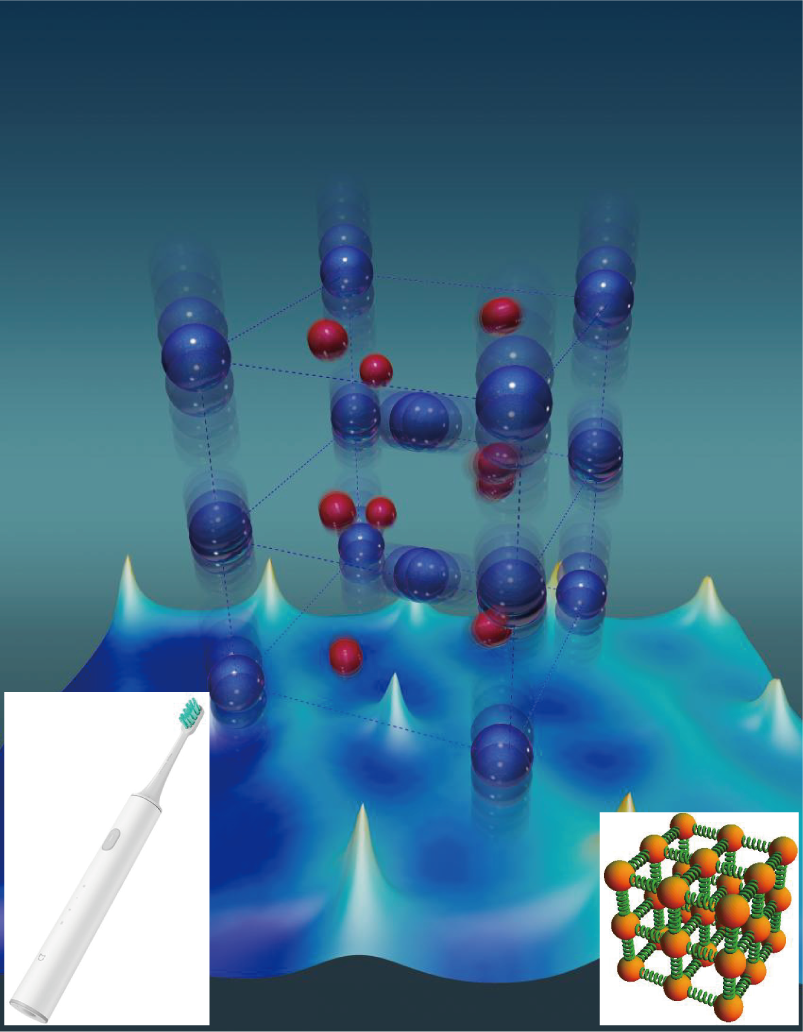
\includegraphics[width=\textwidth]{figure/atomvib.png}
    \end{column}
    \begin{column}{0.5\textwidth}
      \begin{block}{}\begin{itemize}\small
        \item The atoms in the solid are \textcolor{purple}{jiggling} all the time.
        \item The vibration amplitude usually far smaller that the atoms radius, e.g., \textcolor{purple}{\(0.01\sim0.1\)\r{A}}.\footnote{\tiny L. Cartz, Proc. Phys. Soc. B \textbf{68}, 957 (1955).}
        \item The speed or frequency of the atoms' movement is usually in \textcolor{purple}{\( 1\sim 10\)THz} level, much lower that the electrons'.
        \item That vibration of each atom is \textcolor{purple}{not independent}. 
        \item All of the atoms in the solids \textcolor{purple}{vibrate together}, forming an fantastic picture.
      \end{itemize}\end{block}
    \end{column}
  \end{columns}
\end{frame}
%============================================================================

%============================================================================
\begin{frame}{One dimensional atomic chain: describe}\small
  \begin{center}
    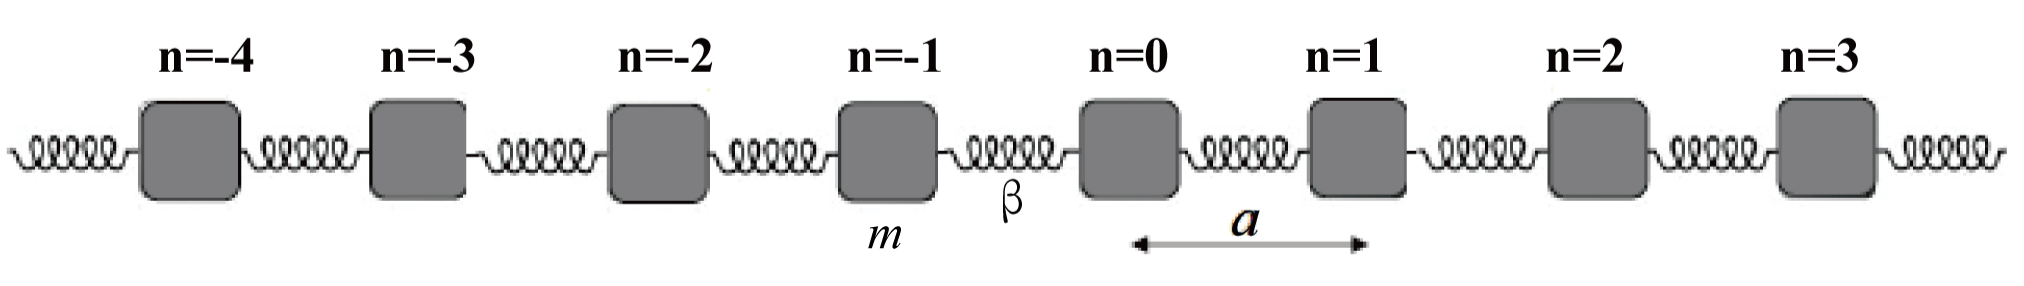
\includegraphics[width=0.95\textwidth]{figure/atom_chain.png}
  \end{center}
  \begin{block}{}
    To discribe the vibration on this atoms chain, we introduce two kinds of parameters: 
    \begin{itemize}
      \item The space frequency \textcolor{purple}{\(q=2\pi/\lambda\)}
      \item The time frequency \textcolor{purple}{\(\omega = 2\pi/T\)}
    \end{itemize}
  \end{block}
  This typical analytical mechanics question has a concise result.
  \begin{subequations}\begin{align}
      u_n &= A\mathrm{e}^{-i(\omega{}t-naq)}\\
      \omega^2 &= \frac{2\beta}{m}[1-\cos(qa)]
  \end{align}\end{subequations}
  Where, \textcolor{purple}{\(u_n\)} is the displacement of the \textcolor{purple}{\(n\)}th atom, \textcolor{purple}{\(\beta = \left.\frac{\partial^2{}V}{\partial{}u_n^2}\right|_{u_n=0}\)}, \textcolor{purple}{\(V\)} is the potential energy around each atoms.
\end{frame}
%============================================================================

%============================================================================
\begin{frame}{One dimensional atoms chain: analysis}\small
  \begin{center}
    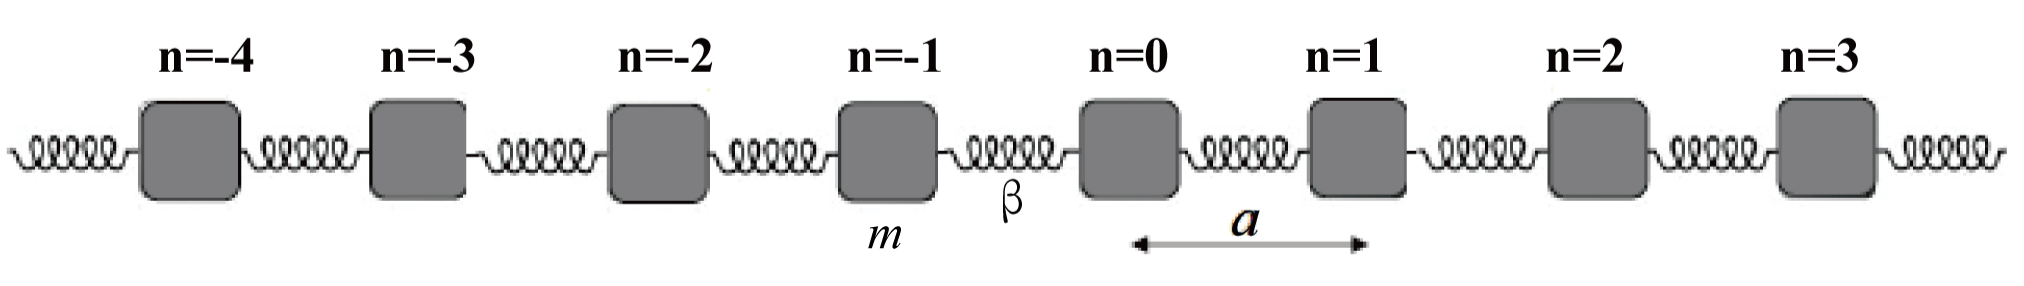
\includegraphics[width=0.95\textwidth]{figure/atom_chain.png}
  \end{center}
  \begin{equation*}\small
      u_n = A\mathrm{e}^{-i(\omega{}t-naq)}, \;\omega = 2\sqrt{\frac{\beta}{m}}\left|\sin\frac{aq}{2}\right|
  \end{equation*}
  \begin{columns}
    \begin{column}{0.35\textwidth}
      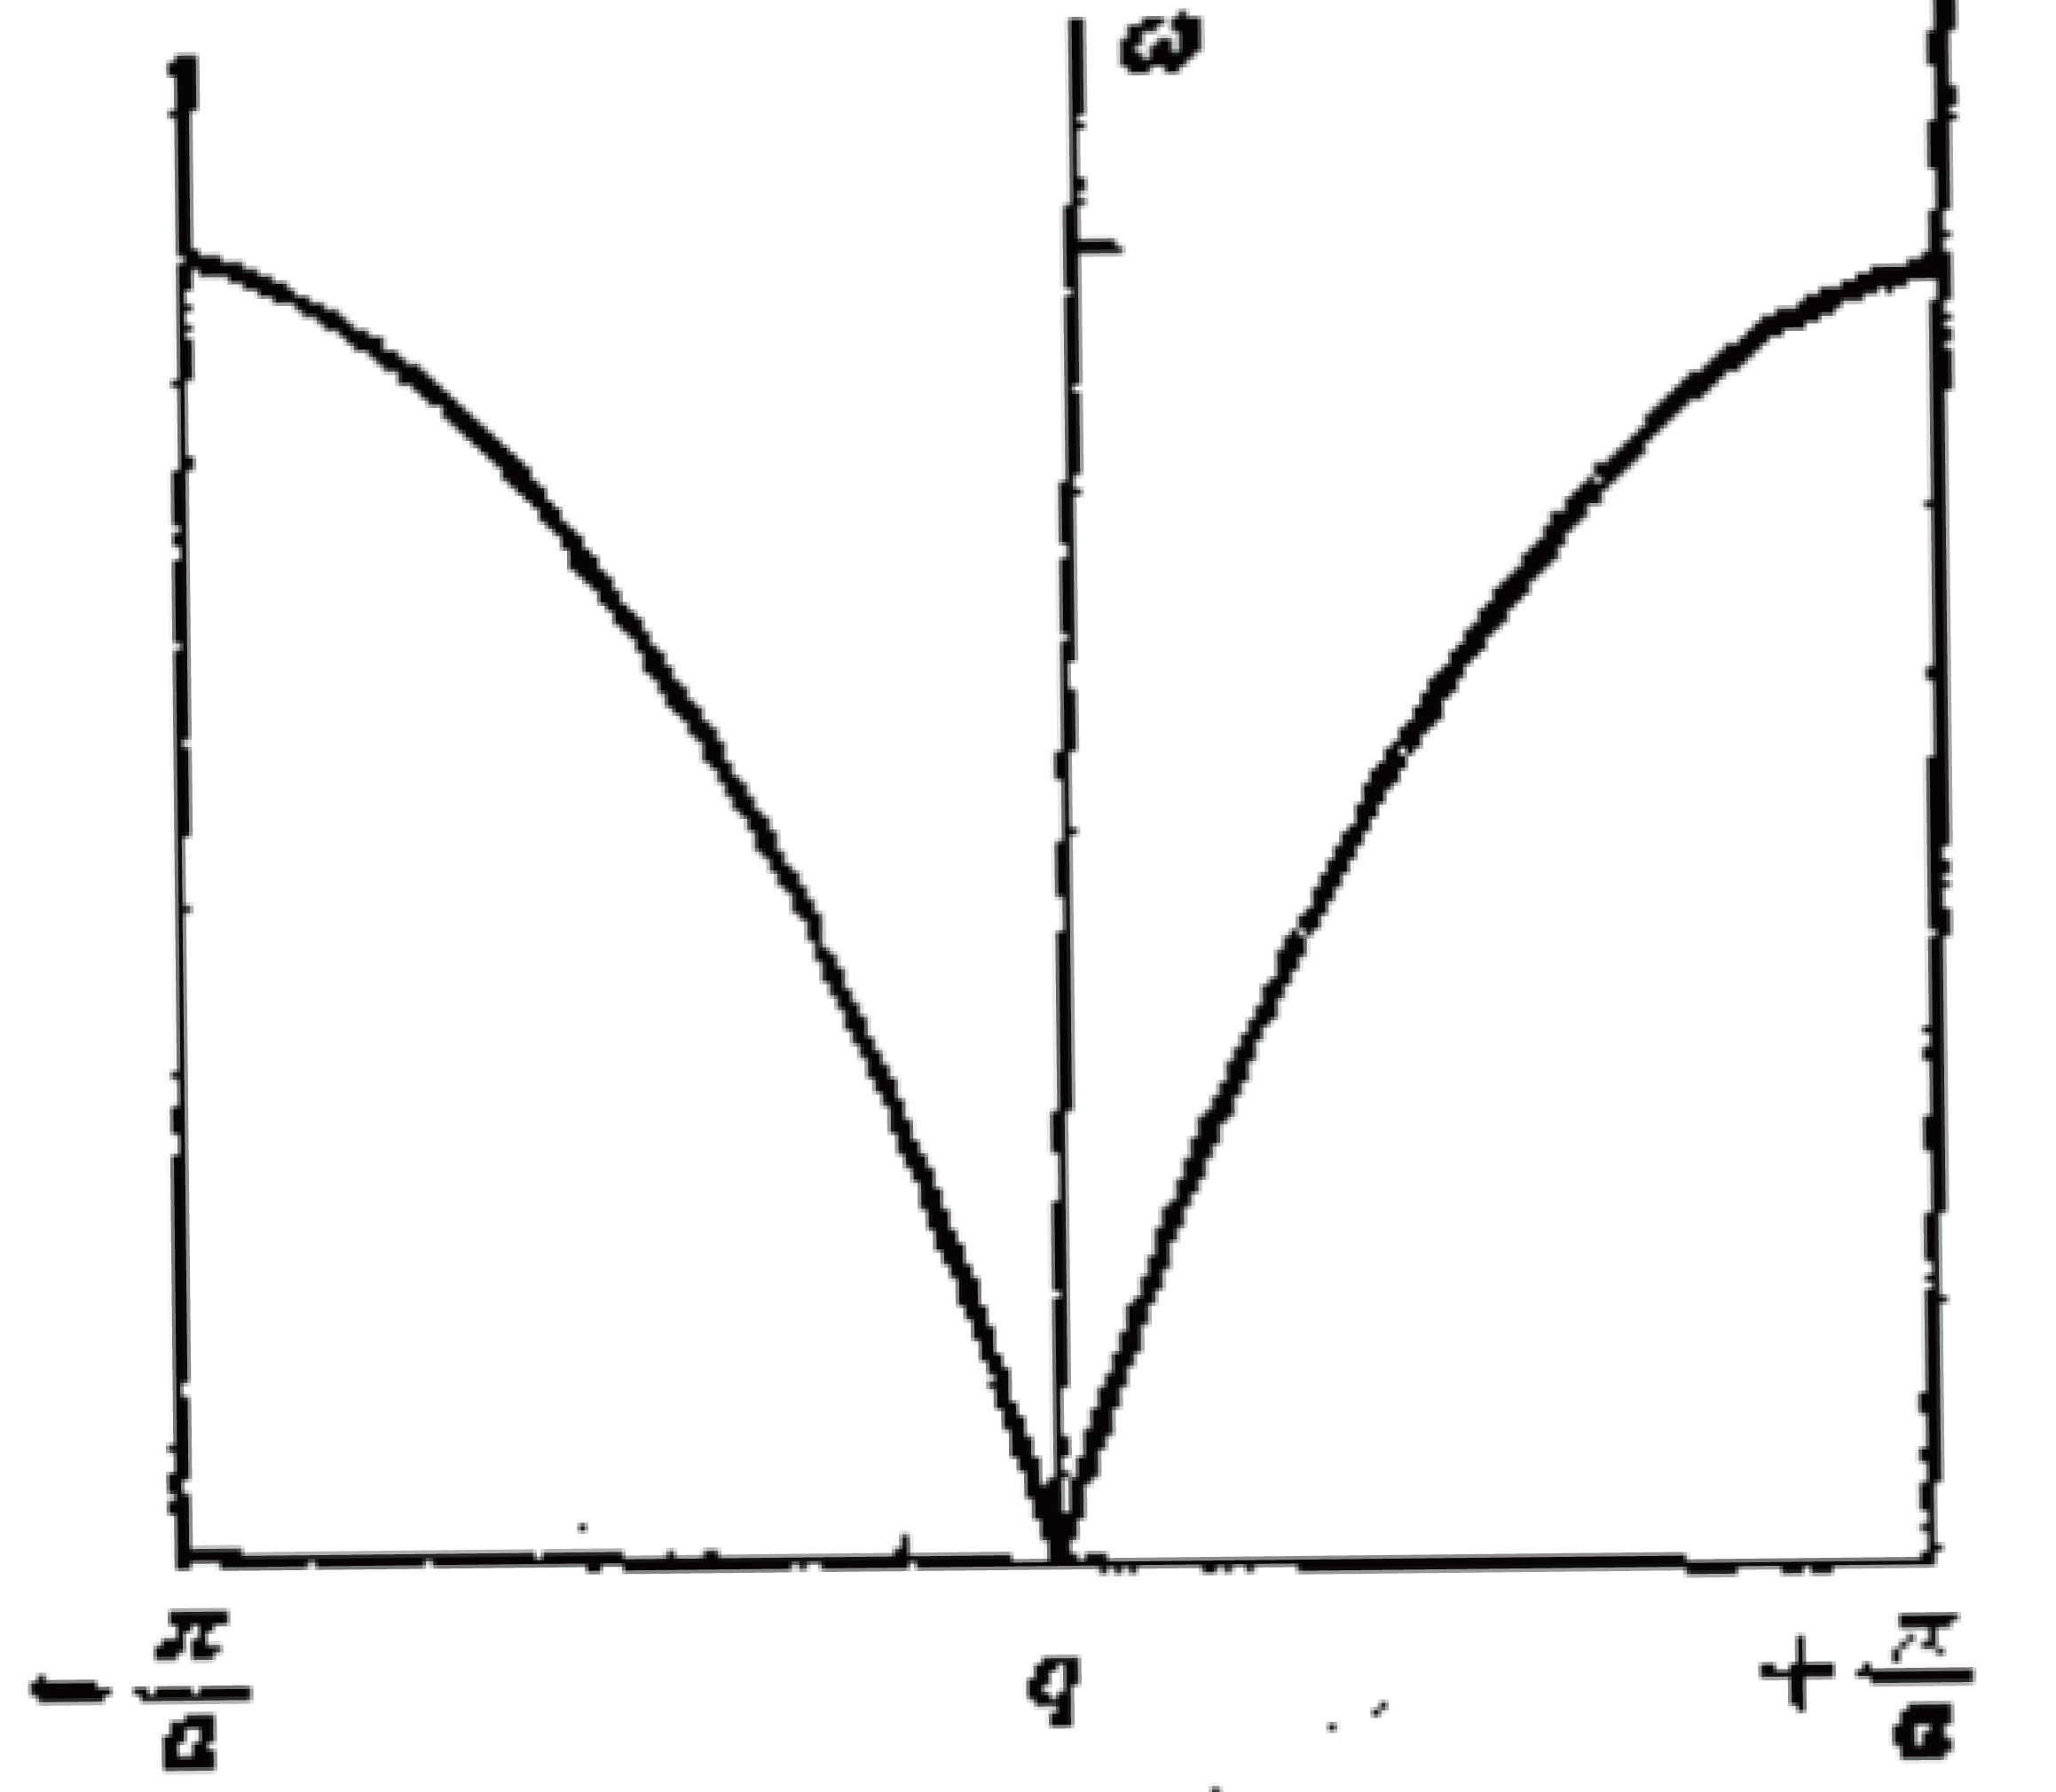
\includegraphics[width=\textwidth]{figure/1dc-solution.png}
    \end{column}
    \begin{column}{0.65\textwidth}
      \begin{block}{}\begin{itemize}\footnotesize
        \item The vibration of each atom follows the \textcolor{purple}{simple harmonic motion} format.
        \item The relation of \(\omega(q)\), which also called 
        ``\textcolor{purple}{dispersion relation}'' or ``\textcolor{purple}{phonon spectrum}'', is periodic in \(q\), with the period of \(2\pi/a\).
        \item The \(\omega\) at \(q=0\) (the \textcolor{purple}{\(\Gamma\)} point) is zero, for it represent a \textcolor{purple}{constant vibration}, means, no inter vibration.
        \item The \(\omega(q)\) near the \(\Gamma\) point shows a \textcolor{purple}{linear dispersion} relation.
      \end{itemize}\end{block}
    \end{column}
  \end{columns}
\end{frame}
%============================================================================

%============================================================================
\begin{frame}{Vibration in continuous medium (Long-wave limit)}
  \begin{columns}
    \begin{column}{0.4\textwidth}
      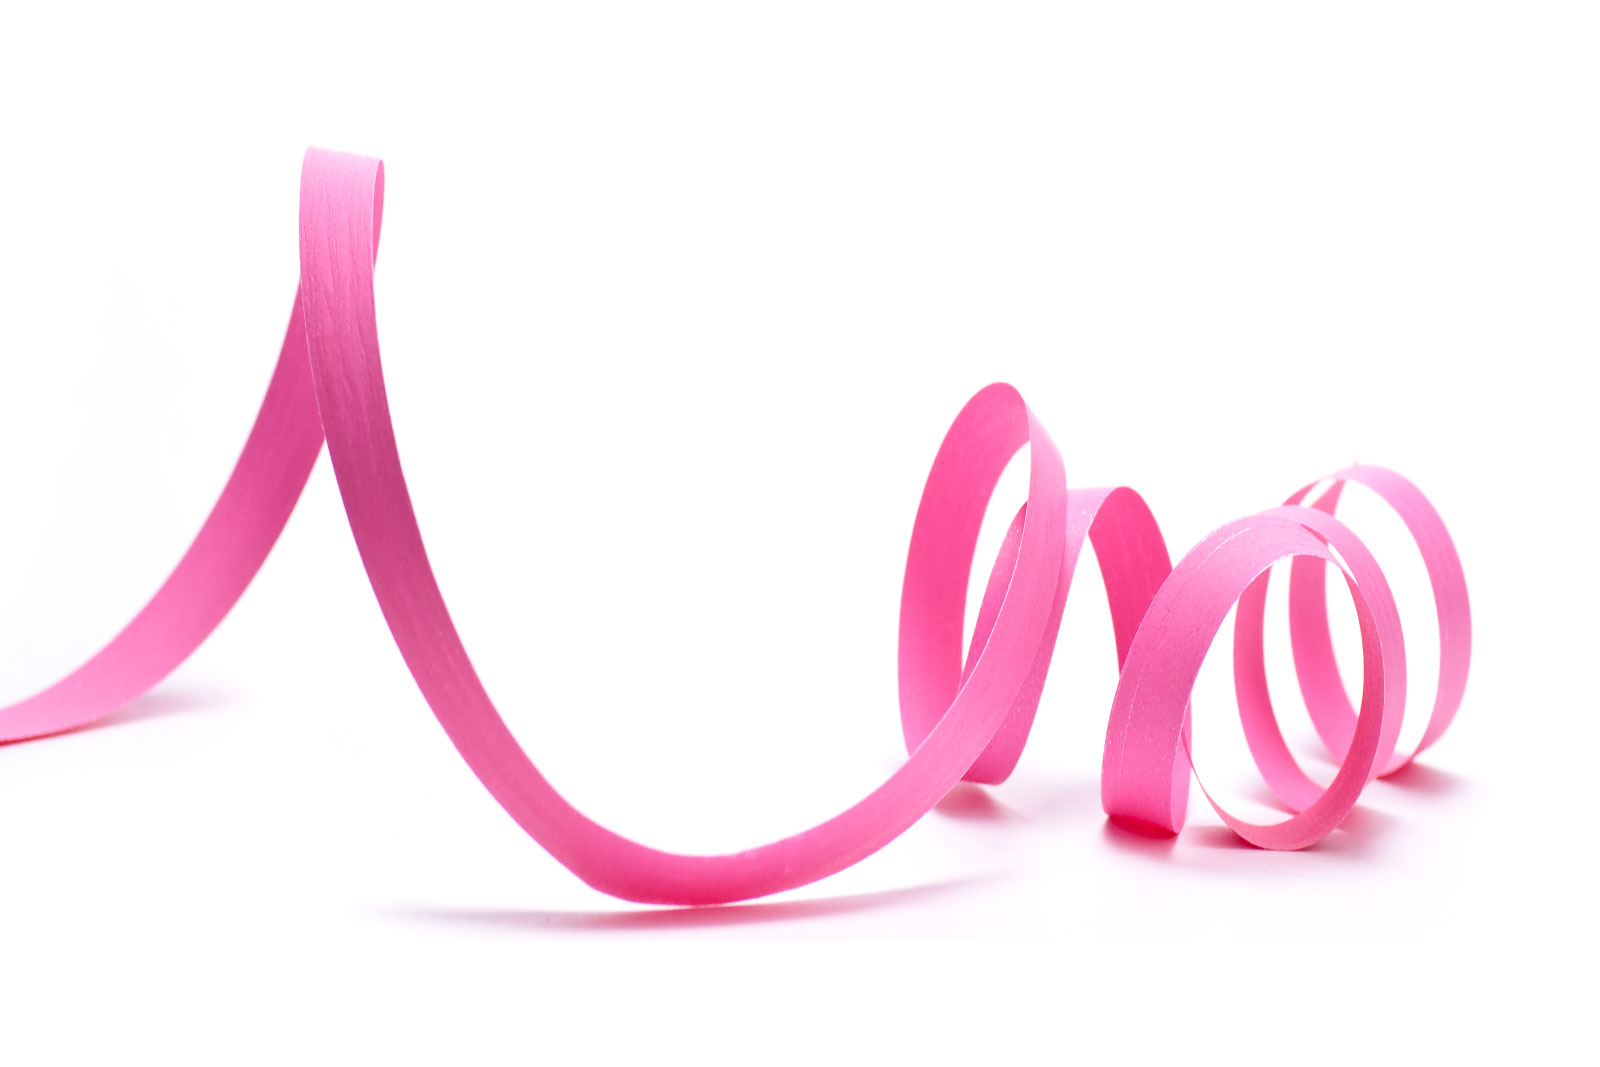
\includegraphics[width=\textwidth]{figure/ribbon.jpg}
    \end{column}
    \begin{column}{0.4\textwidth}
      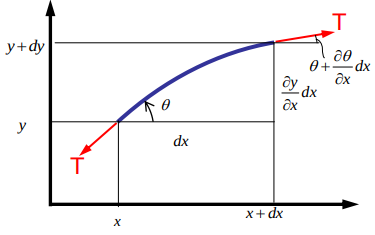
\includegraphics[width=\textwidth]{figure/longwave.png}
    \end{column}
  \end{columns}
  Under the \textcolor{purple}{long-wave limit} (the \(q\) near the \(\Gamma\) point), the lattice wave can be exactly regarded as spreading in a \textcolor{purple}{continuous medium}.

  The vibration in the continuous medium is also a typical analytical mechanics problem.
  \begin{block}{}
    The dispersion relation of \(\omega - q\) has a simple \textcolor{purple}{linear relation}, 
    \begin{equation}
      \omega = vq
    \end{equation}
    Where, \textcolor{purple}{\(v\)} is the group velocity of the wave, a constant.
  \end{block}
  
\end{frame}
%============================================================================

%============================================================================
\begin{frame}{What if primitive cell contains two atoms?}
  \begin{figure}
    \centering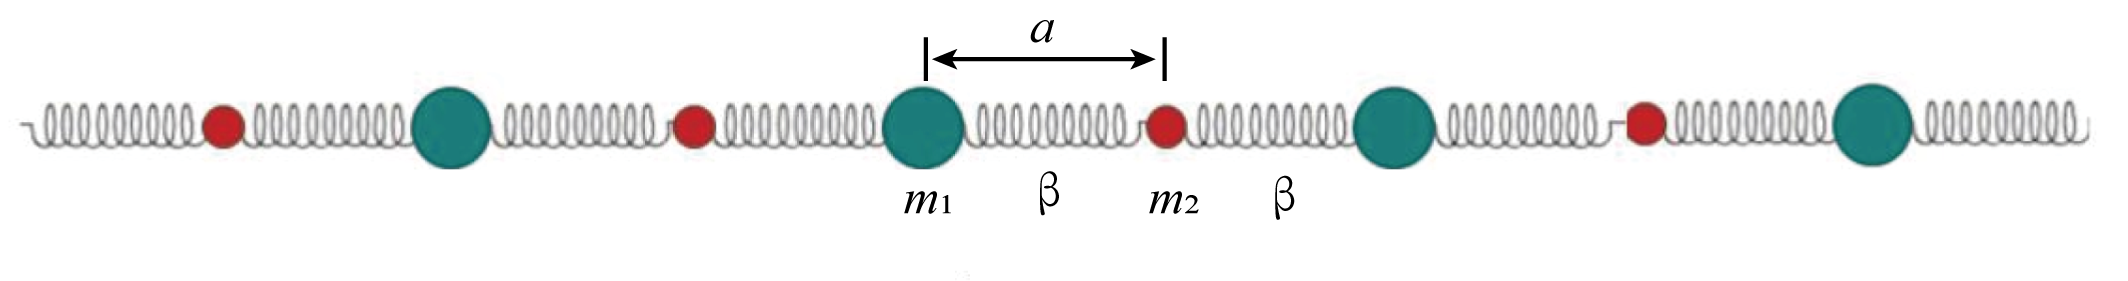
\includegraphics[width=\textwidth]{figure/atom_chain_2.png}
  \end{figure}
  \begin{equation}
      \omega_\pm^2 = \beta\frac{m_1+m_2}{m_1m_2}\left\{1\pm[1-\frac{4m_1m_2}{(m_1+m_2)^2}\sin^2(aq)]^{1/2}\right\}
  \end{equation}
  \begin{columns}
    \begin{column}{0.35\textwidth}
      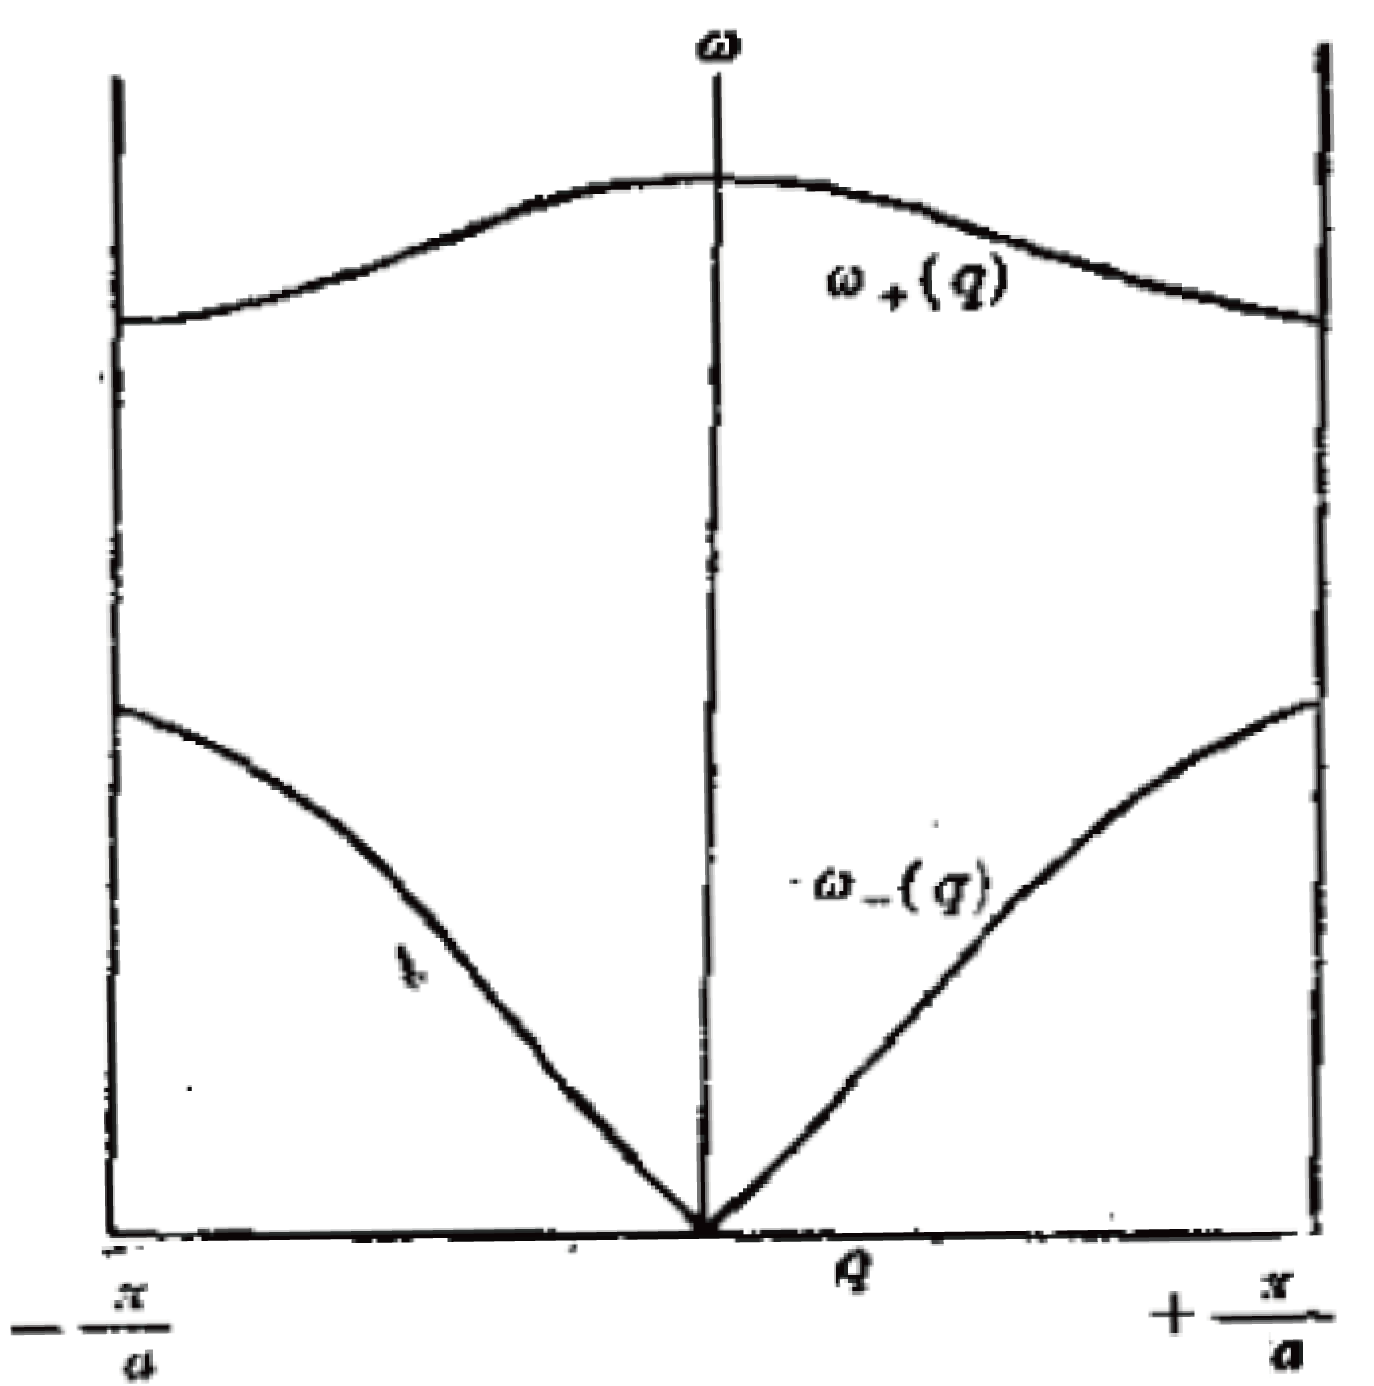
\includegraphics[width=\textwidth]{figure/1dc2-solution.png}
    \end{column}
    \begin{column}{0.65\textwidth}
      \begin{block}{}\begin{itemize}\footnotesize
        \item There are \textcolor{purple}{two kinds of ``branches''} in phonon spectrum. Near the \(\Gamma\) point, the lower branch still shows a linear dispersion, but the upper does not.
        \item We called the lower branch as the \textcolor{purple}{acoustic branch}, and the upper branch as \textcolor{purple}{optical branch}.
        \item In one dimensional system, the \textcolor{purple}{number of the total branches} is equal to the \textcolor{purple}{number of atoms in one primitive cell}.
      \end{itemize}\end{block}
    \end{column}
  \end{columns}
\end{frame}
%============================================================================

%============================================================================
\begin{frame}{Acoustic branch and optical branch}
  \begin{columns}
    \begin{column}{0.2\textwidth}
      \centering
      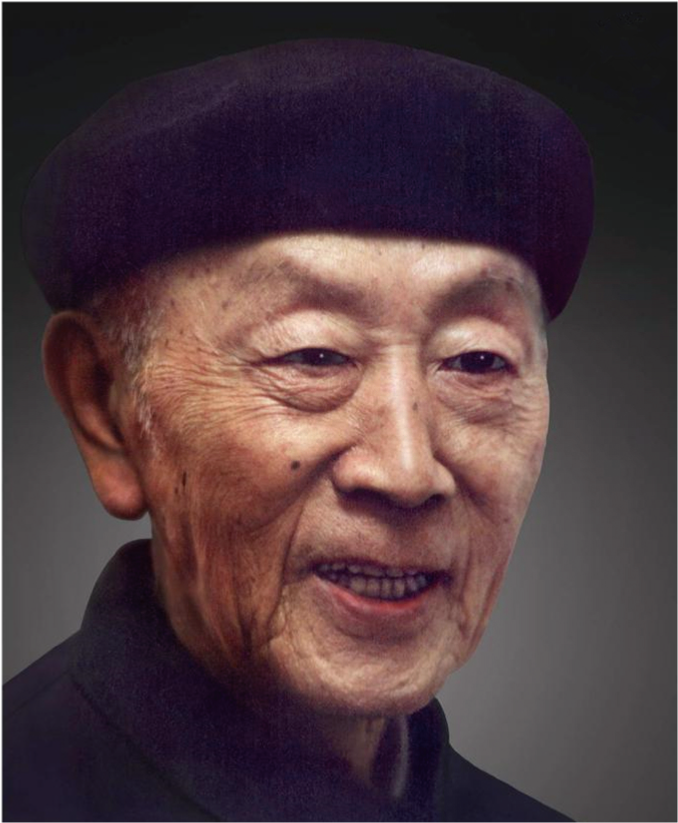
\includegraphics[width=\textwidth]{figure/kunhuang.png}
      {\scriptsize 黄昆 (Kun Huang)}
      \  \\
      \  \\
      \  \\

      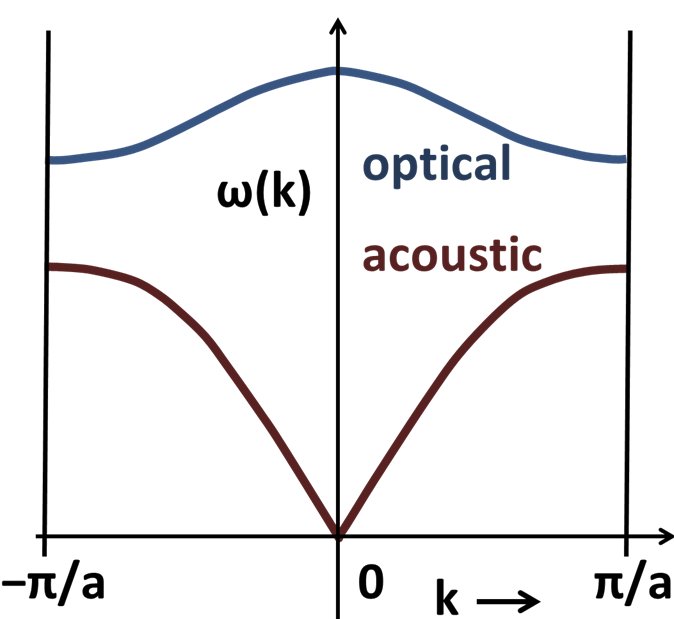
\includegraphics[width=\textwidth]{figure/ao-opt-phon.png}
    \end{column}
    \begin{column}{0.8\textwidth}
      \begin{block}{}
        \begin{itemize}
          \item There are two kinds of branches in the phonon spectrum, \textcolor{purple}{acoustic branch} and \textcolor{purple}{optical branch}.
          \item The \textcolor{purple}{acoustic branch} described the \textcolor{purple}{vibration of the center of mass} for the whole primitive cell.
          \item The \textcolor{purple}{optical branch} described the vibration of atoms in each primitive cell. In the optical mode, the primitive cell's \textcolor{purple}{center of mass DOES NOT move}.
          \item There will be \textcolor{purple}{\(d\) acoustic branch} and \textcolor{purple}{\((n-1)d\) optical branch}, where \(d\) is the space dimension, and \(n\) is the atoms number in one primitive cell.
          \item As prof. Huang points, the energy or frequency of optical modes is higher than the acoustic modes, and the optical brancher near the \(\Gamma\) point do not satisfied the linear dispersion, are all caused by the \textcolor{purple}{electric forces between atoms}.
        \end{itemize}
      \end{block}
    \end{column}
  \end{columns}
\end{frame}
%============================================================================

%============================================================================
\begin{frame}{Phonon spectrum in solids: calculation equation}\scriptsize
  \color{gray} The Hamiltonlian of the phonon system is,
  \begin{equation}
    H = C_0 + \frac{1}{2}\sum_{\mu\alpha{}i}M_\alpha\dot{u}^2_{\mu\alpha{}i} + \frac{1}{2}\sum_{\mu\alpha{}i,\nu\beta{}j}C^{\nu\beta{}j}_{\mu\alpha{}i}u_{\mu\alpha{}i}u_{\nu\beta{}j}
  \end{equation}
  So we get its motion equation,
  \begin{equation}
    M_\alpha\ddot{u}_{\mu\alpha{}i} = -\sum_{\nu\beta{}j}C^{\nu\beta{}j}_{\mu\alpha{}i}u_{\nu\beta{}j}
  \end{equation}
  Let, 
  \begin{equation}
    D_{\alpha\beta,ij}(\bm{q}) = D_{\alpha\beta,ij}(\bm{q}, \mu)= \sum_\nu\frac{1}{\sqrt{M_\alpha{}M_\beta}}C^{\nu\beta{}j}_{\mu\alpha{}i}\mathrm{e}^{i\bm{k}\cdot(\bm{R}_\nu-\bm{R}_\mu)}
  \end{equation}
  And the phonon spectrum \(\omega(\bm{q})\) can be calculated as,
  \begin{equation}
    \label{eq::ph}
    \mathrm{det}|\omega^2\delta_{\alpha\beta}\delta_{ij}-D_{\alpha\beta,ij}(\bm{q})| = 0
  \end{equation}
  Where \(\mu,\nu\) are the index of primitive cells, \(\alpha,\beta\) are the index of atoms in each primitive cell, and \(i,j\) are the index of directions.
\begin{block}{}
  \color{black} The key parameters we need for calculate the phonon spectrum is the \textcolor{purple}{force constant matrix} \(\bm{C} = [C^{\nu\beta{}j}_{\mu\alpha{}i}]\). \textcolor{purple}{\(C^{\nu\beta{}j}_{\mu\alpha{}i}\)} means that, if the \textcolor{purple}{\(\beta\)}th atom in \textcolor{purple}{\(\nu\)}th cell move a unit length in \textcolor{purple}{\(j\)} direction, what forces will the \textcolor{purple}{\(\alpha\)}th atom in \textcolor{purple}{\(\mu\)}th cell in \textcolor{purple}{\(i\)} direction fell.
\end{block}
\end{frame}
%============================================================================

%============================================================================
\begin{frame}{Phonon spectrum in solids: LA, LO, TA, TO}\small
  \begin{center}
    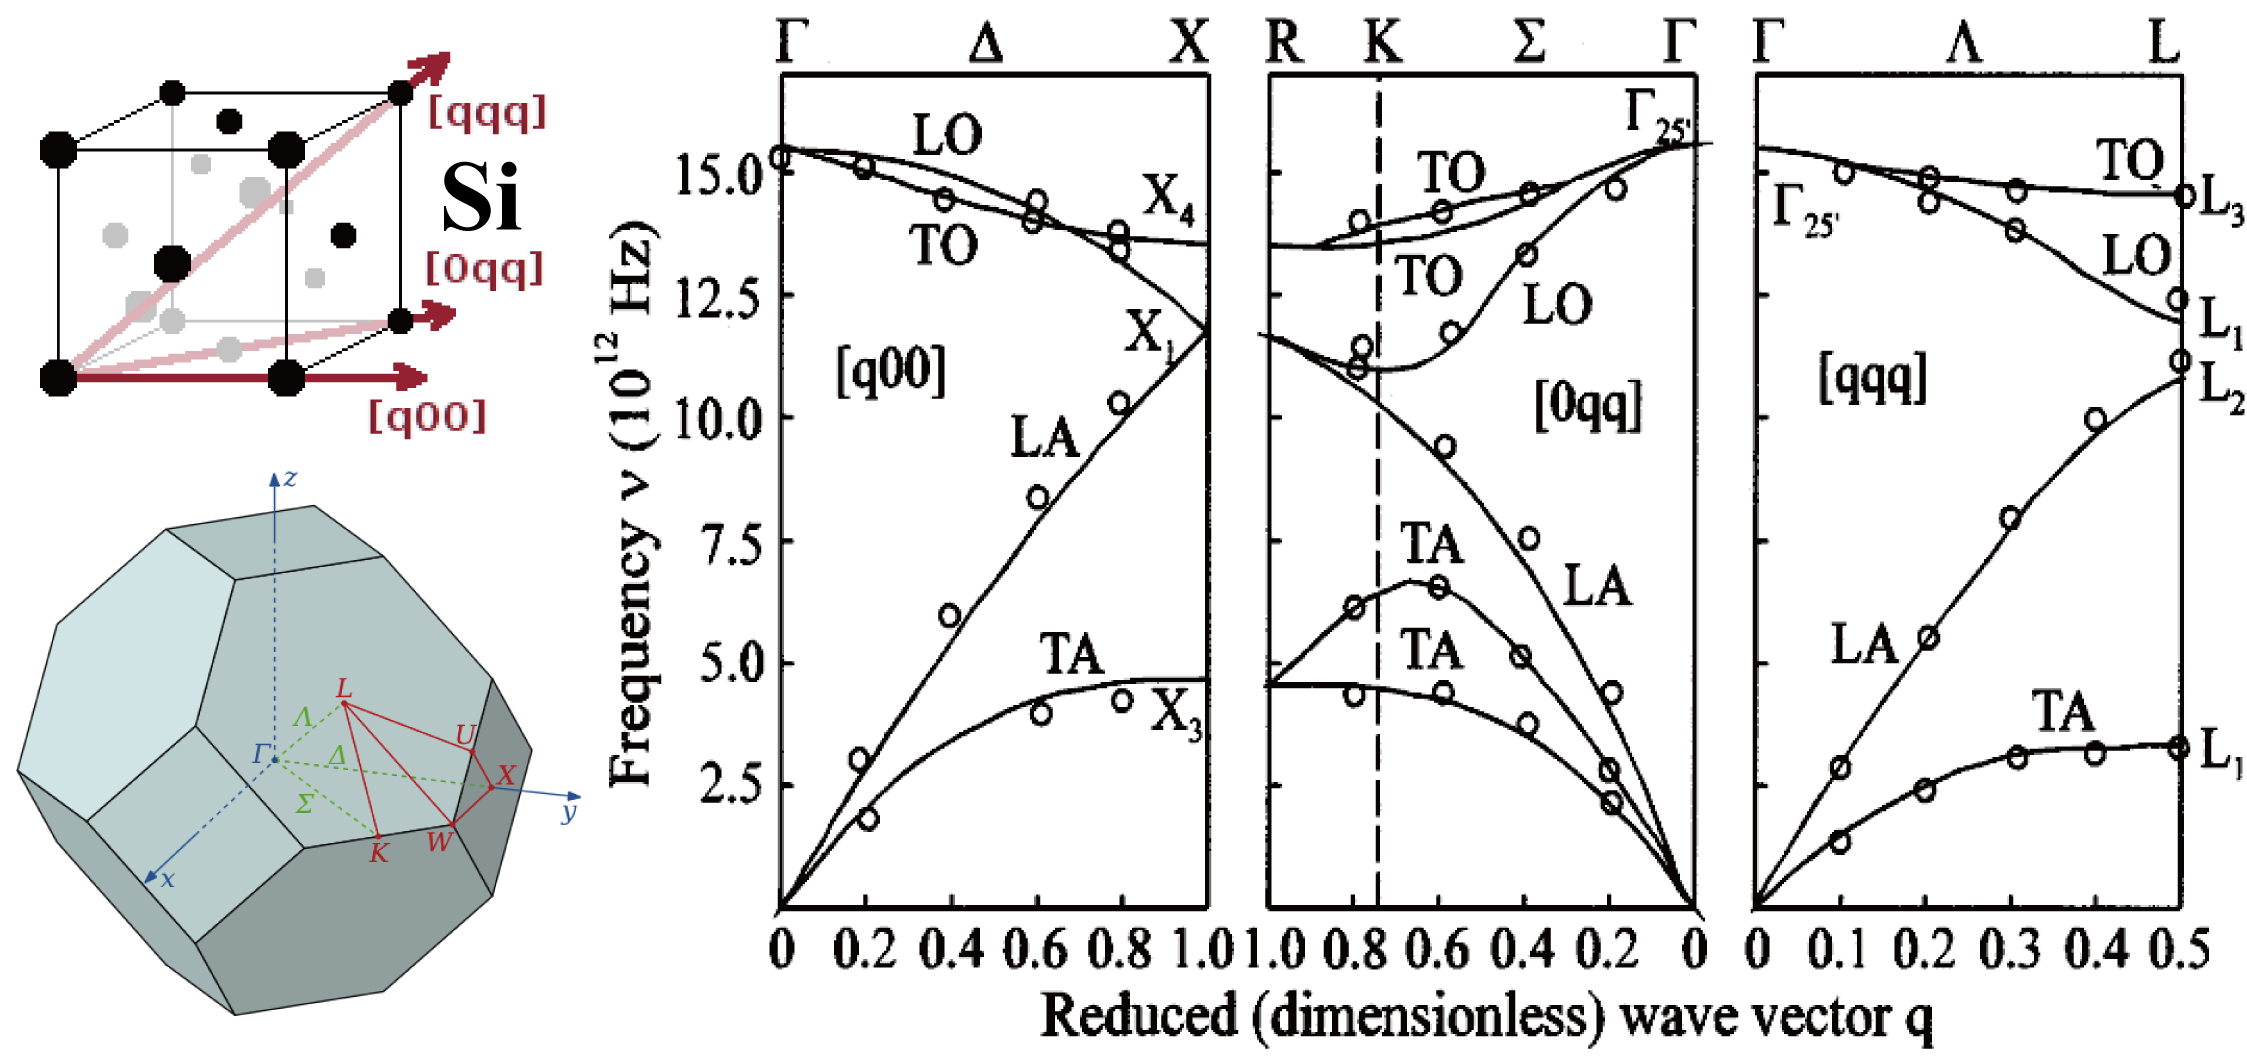
\includegraphics[width=0.8\textwidth]{figure/ps-solid.png}\\
    \tiny R. Tubino, \emph{et. al.}, J. Chem. Phys. \textbf{56}, 1022 (1972).
  \end{center}
  \begin{block}{}
    \begin{itemize}\footnotesize
      \item For each direction, there are \textcolor{purple}{acoustic} and \textcolor{purple}{optical branches}.
      \item Both kinds of branches split into \textcolor{purple}{longitudinal} and \textcolor{purple}{transversal} modes (longitudinal acoustic (\textcolor{purple}{LA}) and optical (\textcolor{purple}{LO}) and transversal acoustic (\textcolor{purple}{TA}) and optical (\textcolor{purple}{TO})).
      \item In some cases, the transversal branches \textcolor{purple}{split further}.
    \end{itemize}
  \end{block}
\end{frame}
%============================================================================

%============================================================================
\begin{frame}{Imaginary frequency in phonon spectrum}
\begin{columns}
  \begin{column}{0.4\textwidth}
    \begin{center}
      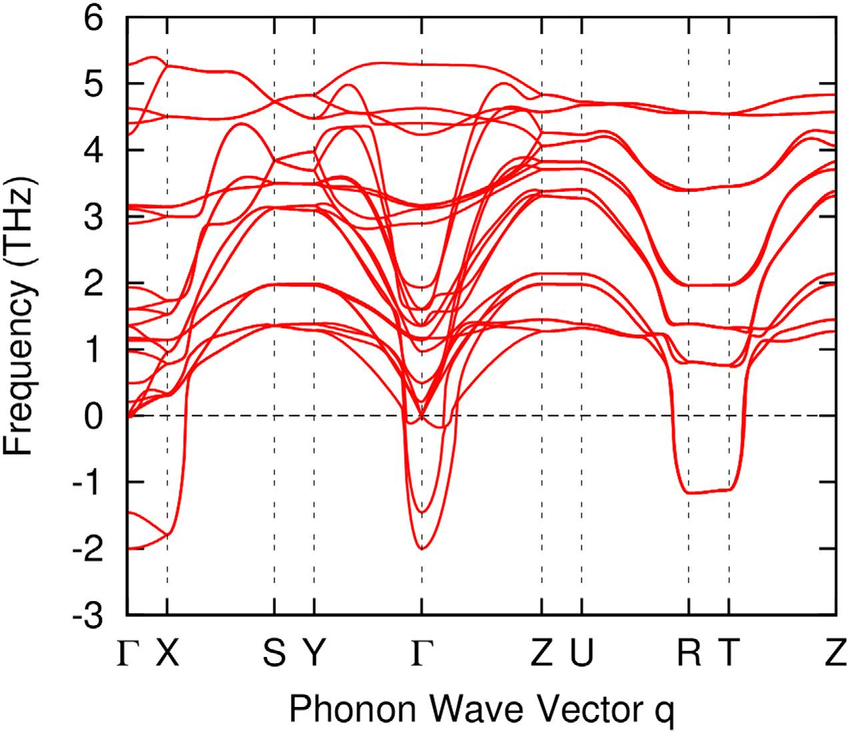
\includegraphics[width=\textwidth]{figure/ps-im.png}
    \end{center}
  \end{column}
  \begin{column}{0.6\textwidth}
    \begin{block}{}
      \begin{itemize}\footnotesize
        \item In some cases, we may get this kind of phonon spectrum in calculation, which has the \textcolor{purple}{``negative''} valued \(\omega\). 
        \item But actually, the \(\omega(\bm{q})\) in the calculation cannot be negative, since we can only get the \textcolor{purple}{\(\omega^2\)} from Eq. \eqref{eq::ph}, and then choice the \textcolor{purple}{positive \(\omega\)}.
        \item The ``negative'' values here actually represent the \textcolor{purple}{imaginary part} of the \(\omega\). In order to express more easily and directly, we \textcolor{purple}{bend them into the real negative plane}.
        \item The appearance of the imaginary part indicates the structure's \textcolor{purple}{dynamic instability}. Because,
        \begin{equation}\scriptsize
          u_{\mu\alpha{}i}(\bm{q},t) = \frac{\bm{e}_{\alpha{}i}(\bm{q})}{\sqrt{M_\alpha}}\mathrm{e}^{-i(\omega{}t-\bm{q}\cdot\bm{R}_\mu)} = \bm{A}_{\mu\alpha{}i}\mathrm{e}^{-i\omega{}t}
        \end{equation}
      \end{itemize}
    \end{block}
  \end{column}
\end{columns}
\end{frame}
%============================================================================

\section{Calculation Methods}

%============================================================================
\begin{frame}{Force constant matrix in solid}
  \begin{columns}
    \begin{column}{0.6\textwidth}
      As we mention before, the key parameters we need for calculating the phonon spectrum is the \textcolor{purple}{force constant matrix} \(\bm{C} = [C^{\nu\beta{}j}_{\mu\alpha{}i}]\) (\(\bm{\Phi}\) in the figure). 
  The \(\bm{C}\) has at least two different meaning, 
  \begin{itemize}
    \item The \textcolor{purple}{forces} that other atoms might feel if we move one atom.
    \item The \textcolor{purple}{second derivative of potential energy} about position. \(C^{\nu\beta{}j}_{\mu\alpha{}i} = \left.\frac{\partial^2V}{\partial{}u_{\mu\alpha{}i}\partial{}u_{\nu\beta{}j}}\right|_{u=0}\) 
     \end{itemize}
    \end{column}
    \begin{column}{0.4\textwidth}
      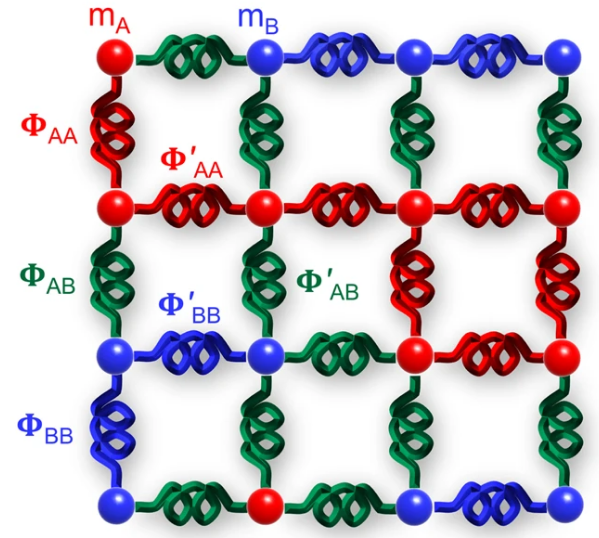
\includegraphics[width=\textwidth]{figure/fc.png}
    \end{column}
  \end{columns}
  \begin{block}{}
    In order to get \(\bm{C}\), rather than using the empirical potential or simple Coulomb forces between atoms, we need to use \textcolor{purple}{density functional theory (DFT)} to get precise value of the \textcolor{purple}{forces} or \textcolor{purple}{energies}.
  \end{block}
\end{frame}
%============================================================================

%============================================================================
\begin{frame}{``Frozen phonon method''}
  \begin{block}{}
    The algorithm that the ``frozen phonon method'' use is as follow:
  \begin{itemize}
    \item Read in a target atomic structure, \(\bm{S}\).
    \item \textcolor{purple}{Slightly change the position} of one atom in \(\bm{S}\), get a new atomic structure, \(\bm{S}'_1\).
    \item Use \textcolor{purple}{DFT method} calculate \(\bm{S}'_1\), and obtain the forces on all of the atoms.
    \item Slightly change the position of \textcolor{purple}{another atom} in \(\bm{S}\), get another new atomic structure, \(\bm{S}'_2\). Repeat steps above.
    \item \textcolor{purple}{Summarize} all of the forces in all of the structures, calculate the phonon spectrum.
  \end{itemize}
  \end{block}
  \begin{center}
    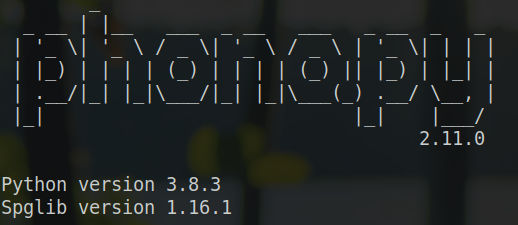
\includegraphics[width=0.42\textwidth]{figure/phonopy.png}
  \end{center}
\end{frame}
%============================================================================

\section{Phonon Spectrum of LuFe\(_2\)O\(_{4.86}\)}

%============================================================================
\begin{frame}{Difficulties in complex magnetic system}
  \begin{block}{}
    In the \textcolor{purple}{complex magnetic system}, obtain the \textcolor{purple}{stable phonon spectrum} using ``frozen phonon method'' may \textcolor{purple}{face some challenges},
  \begin{itemize}
    \item The slight movement of atoms may let the DFT calculation fall into a \textcolor{purple}{meta-stable state}, especially when the system is magnetic or extremely complex.
    \item Even worse, in a large system, randomly move one atom may cause the DFT calculation \textcolor{purple}{hard to converge}.
    \item The phonon spectrum is \textcolor{purple}{extremely expensive} in time and resources when we try to calculate a huge system, for it may contain hundreds of calculation tasks.
  \end{itemize}
  \end{block}
\end{frame}
%============================================================================

%============================================================================
\begin{frame}{LuFe\(_2\)O\(_{4.86}\) without electron/hole doping}
\begin{columns}
  \begin{column}{0.5\textwidth}
    \centering
    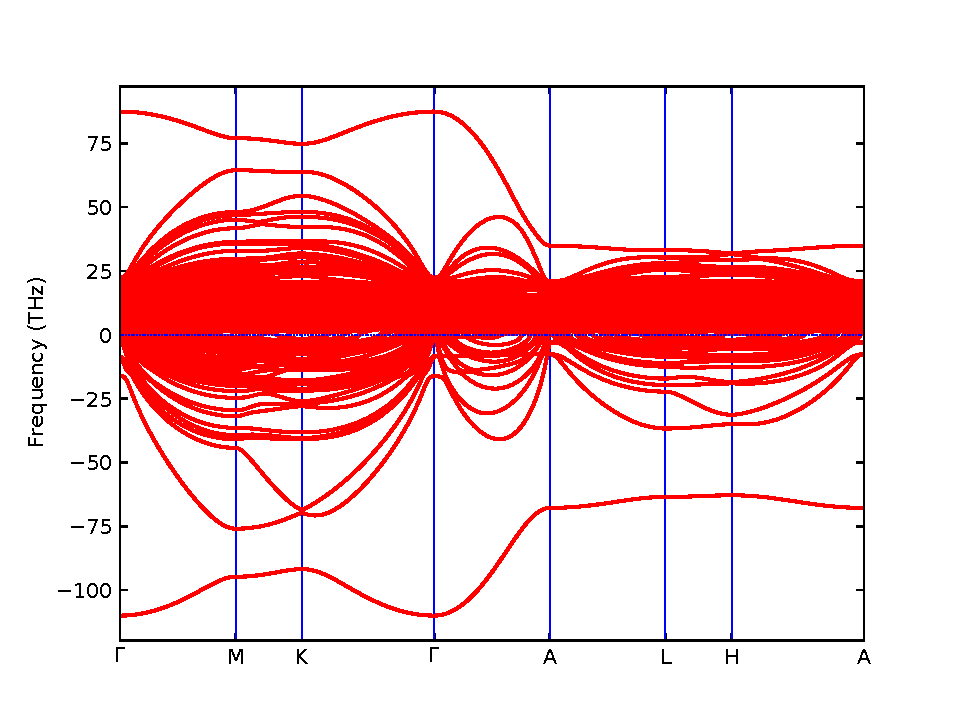
\includegraphics[width=\textwidth]{figure/wI-e0.pdf}
    \scriptsize With inversion without hole doping
  \end{column}
  \begin{column}{0.5\textwidth}
    \centering
    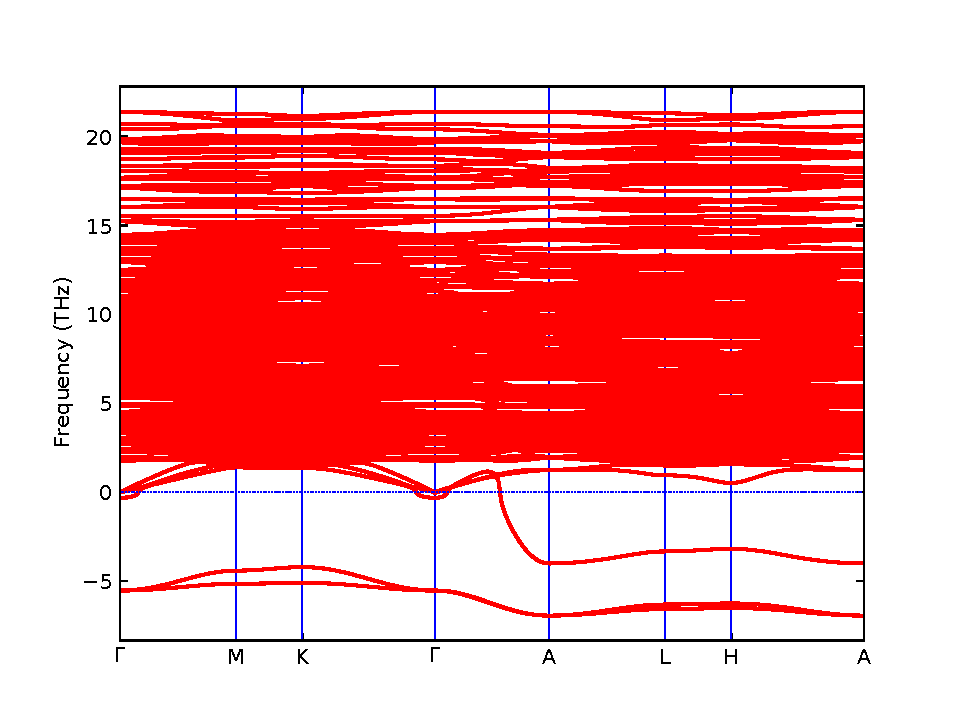
\includegraphics[width=\textwidth]{figure/woI-e0.pdf}
    \scriptsize Without inversion without electron doping
  \end{column}
\end{columns}
\begin{block}{}
  Without any electron or hole doping, the phonon spectrum is \textcolor{purple}{unstable}.
\end{block}
\end{frame}
%============================================================================

%============================================================================
\begin{frame}{LuFe\(_2\)O\(_{4.86}\) with electron/hole doping}
  \begin{columns}
    \begin{column}{0.5\textwidth}
      \centering
      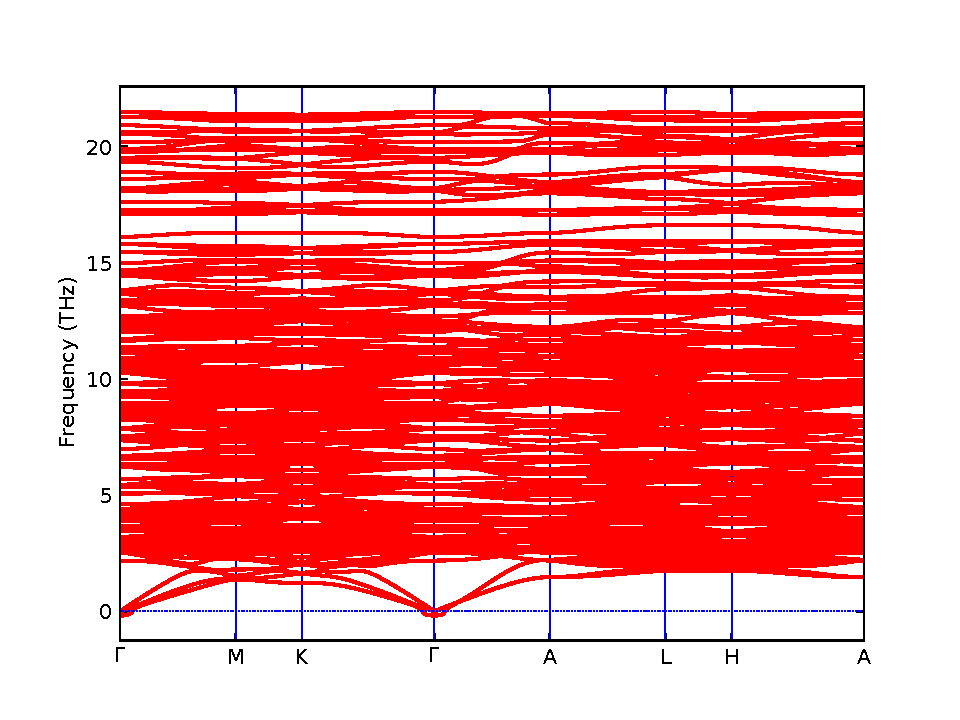
\includegraphics[width=\textwidth]{figure/wI-h1.pdf}
      \scriptsize With inversion with one-hole doping
    \end{column}
    \begin{column}{0.5\textwidth}
      \centering
      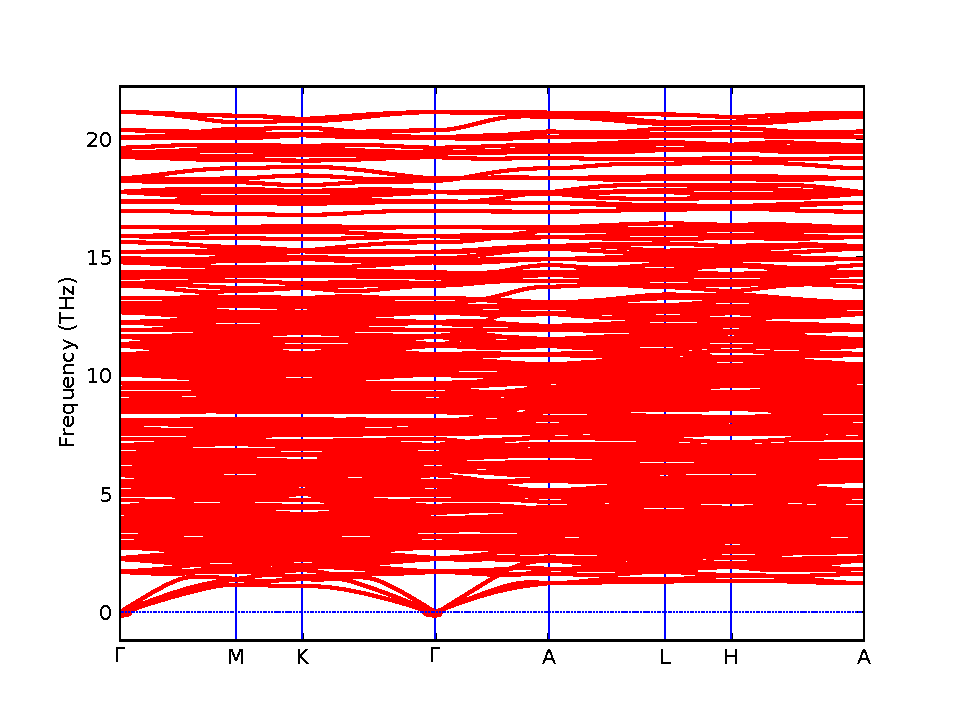
\includegraphics[width=\textwidth]{figure/woI-e1.pdf}
      \scriptsize Without inversion with one-electron doping
    \end{column}
  \end{columns}
  \begin{block}{}
    With electron or hole doping, the phonon spectrum is \textcolor{purple}{stable}. The tiny imaginary parts near the \(\Gamma\) point is some numerical error, which are usually ignored.
  \end{block}
\end{frame}
%============================================================================
\end{document}
